\documentclass{article}
\author{
  Torrent Gorjon, Xavier\\
  \texttt{Xavier.TorrentGorjon@os3.nl}
}
\title{InterNetworking and Routing}

\usepackage{graphicx}

\usepackage[backend=bibtex]{biblatex}

\bibliography{references}


\begin{document}


\begin{titlepage}
\center
\textsc{}\\[1cm]
\textsc{\LARGE University of Amsterdam}\\[1.5cm]

\textsc{\Large InterNetworking and Routing}\\[0.5cm]


\includegraphics[scale=1]{images/uva.png}\\[3cm]


\begin{minipage}{0.4 \textwidth}
\begin{center}
Xavier Torrent Gorj\'{o}n \\
\emph{Xavier.TorrentGorjon@os3.nl}\\[0.5cm]
\end{center}
\end{minipage}
\hfill

{\large \today} 


\end{titlepage}


\newpage

\tableofcontents

\newpage

\section{Overview}


\subsection{OSI Model}

\begin{center}
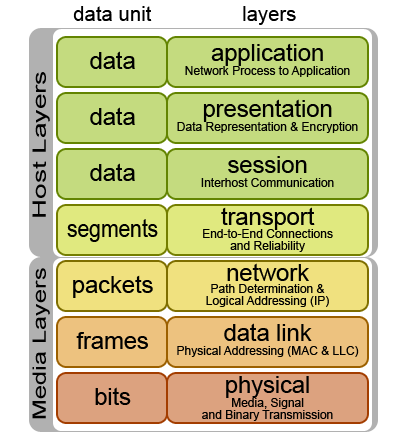
\includegraphics[scale=0.7]{images/OSI-model.png}\\[1cm]
\end{center}


\subsection{Interfaces and Protocols}

\begin{description}
	\item[Interfaces] Interfaces connect different layers on the same computer. Uses Protocol Data Units (PDU).
	\item[Protocols] Protocols are used to communicate between parties data on a specific layer. Uses Service Data Units (SDU) inside Service Access Points (SAP).
\end{description}


\subsection{Encapsulation and Multiplexing}

\begin{description}
	\item[Encapsulation] When data units go down one level in the layer model, headers are added to add information regarding the current layer.
	\item[Multiplexing] Multiple protocols can coexist on the same layer. However, when going down the layer model, these protocols should be treated equally. For example, TCP and UDP are multiplexed down at the IP level, and demultiplexed back when reading the information of IP packets.\footnote{\url{http://www.tcpipguide.com/free/t_TCPIPProcessesMultiplexingandClientServerApplicati-2.htm}}
\end{description}


\subsection{ES Models: Strong vs Weak}

\begin{description}
	\item[Strong ES Model] Hosts suppress packets with a destination address that references another of its interfaces.
	\item[Weak ES Model] Hosts accept packets that match with one of its interfaces addresses, even if it does not receive it on that interface.
\end{description}


\subsection{IP Addressing (IPv4)}

\begin{itemize}
	\item 32-bit addresses
	\item Decimal-dotted notation (a.b.c.d, 0 $=<$ a,b,c,d $=<$ 255).
	\item Special addresses:
	\begin{description}
		\item[0.0.0.0] IP address unknown.
		\item[127.0.0.1] Loopback address.
		\item[Host part all 0] Subnet identifier.
		\item[Host part all 1] Directed broadcast.
		\item[255.255.255.255] Local subnet broadcast.
	\end{description}
	\item Private addresses:
	\begin{description}
		\item[10.0.0.0/8] 
		\item[172.16.0.0/12]
		\item[192.168.0.0/16]
		\item[169.254.0.0/16]
	\end{description}
\end{itemize}


\subsection{Subnetting}

\begin{itemize}
	\item Originally classful subnetting (subnets in A/B/C ranges, with 24, 16 and 8 bits of network addresses respectively; D range for multicast and an unused E range).\footnote{\url{http://en.wikipedia.org/wiki/Classful_network#Introduction_of_address_classes}}
	\item Classless Inter-Domain Routing (CIDR), with network masks to mark the difference between network address and host address. Routing done by selecting most specific match.
	\item Variable Length Subnet Masks (VLSM) to use different subnets that do not have the requirement of having the same size. Add the possibility of subnets inside subnets. This was not possible in RIPv1.
	\item A "link" is defined as the topological area in which a packet with $TTL=1$ can be delivered (aka. not being forwarded).
	\item A "subnet" is the topological area in which the interfaces receive the same network prefix.
\end{itemize}


\subsection{IP Packet Format}

\begin{center}
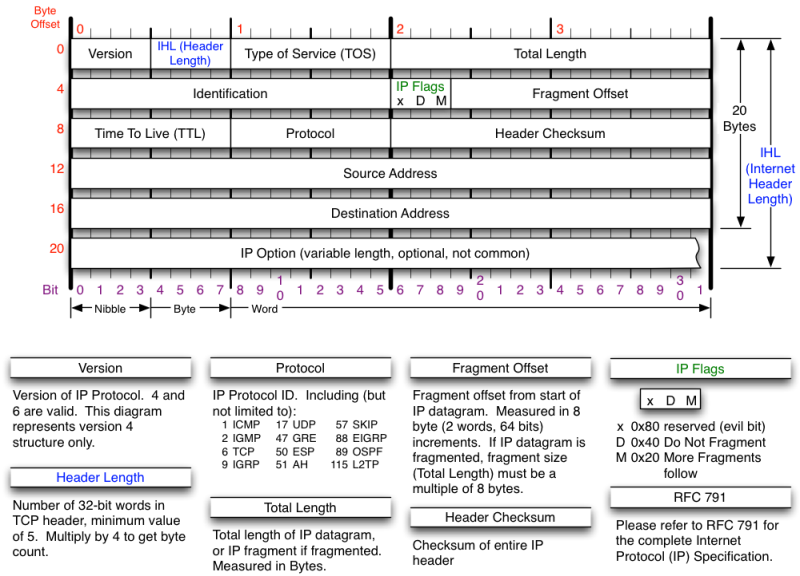
\includegraphics[scale=0.7]{images/IP-Header.png}\\[1cm]
\end{center}

\newpage







\section{CLEAN: Calculating, Legacy, Endianness, Addressing, Networks}

\subsection{Calculating: Counting}

\begin{description}
	\item[Counting] Process that starts with $n=0$ as the initial count. Every counted object is labeled with the actual $n$ value, and n is updated to $n=n+1$. Process ends when all objects have been counted.
\end{description}
	
	
\subsection{Legacy}

\begin{itemize}
	\item Everybody knows what Karst thinks of legacy.
\end{itemize}


\subsection{2-adic vs Binary}

\begin{center}
  \begin{tabular}{ | c | c | c | c | }
    2-adic & Binary & 2-adic to base-10 & Binary to base-10 \\ \hline
    1 & 0 & 1 & 0 \\ \hline
    2 & 1 & 2 & 1 \\ \hline
    11 & 00 & 3 & 0 \\ \hline
    12 & 01 & 4 & 1 \\ \hline
    21 & 10 & 5 & 2 \\ \hline
    22 & 11 & 6 & 3 \\ \hline
    111 & 000 & 7 & 0 \\ 
    \hline
  \end{tabular}
\end{center}

\begin{itemize}
	\item The whole point is that binary resets at every range increase.
\end{itemize}


\subsection{Big-endian and Little-endian}

\begin{center}
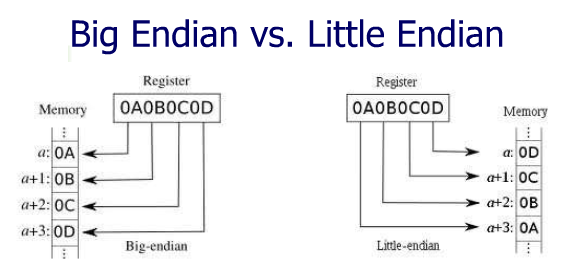
\includegraphics[scale=0.5]{images/BI-LI.png}\\[1cm]
\end{center}


\subsection{Addressing}

\begin{itemize}
	\item \url{http://www.exploringbinary.com/binary-converter/}
\end{itemize}


\newpage







\section{IPv6}


\subsection{Rationale}

\begin{itemize}
	\item $4x$ address space size increase $=$ $2^{96}$ address number increase.
	\item Headers have a fixed size of 40 bytes. Supports extended headers for additional functionality.
	\item NATs no longer needed due the vast amount of addresses.
\end{itemize}


\subsection{Addressing}

\begin{itemize}
	\item 128-bit addresses.
	\item 8 blocks of 4 nibbles ($8x4x4 = 128$ bits)
	\item Consecutive blocks of all-zeroes can be replaced by $::$ once.
	\item No broadcasts, no subnet masks.
	\item \url{http://www.iana.nl/assignments/ipv6-address-space/ipv6-address-space.xhtml}
\end{itemize}


\begin{description}
	\item[Reserved addresses]
\end{description}
	\begin{center}
	\begin{tabular}{ | c | c | }
		\hline
		::/8 & Special-purpose \\ \hline
		100::/8 & Special-purpose \\ \hline
		2000::/3 & Global unicast \\ \hline
		fc00::/7 & Unique local unicast \\ \hline
		fe80::/10 & Link-local (Link-scoped) unicast \\ \hline
		ff00::/8 & Multicast \\
		\hline
	\end{tabular}
	\end{center}

\begin{description}
	\item[Special-purpose addresses]
\end{description}
	\begin{center}
  	\begin{tabular}{ | c | c | }
    	\hline
		::/128 & Unspecified address \\ \hline
		::1/128 & Localhost address \\ \hline
		::a.b.c.d/128(from ::/96) & IPv4-compatible addresses \\ \hline
		::ffff:a.b.c.d/128 (from ::ffff:0:0/96) & IPv4-mapped addresses \\ \hline
		64:ff9b::/96 & Well-known prefix \\ \hline
		100::/64 & Discard-only address block \\
		\hline
	\end{tabular}
	\end{center}
	
	
\subsection{Neighbour Discovery Protocol (NDP)}
	
\begin{itemize}
	\item IPv6 does not use ARP. Uses ICMPv6 instead.
	\item ICMPv6 types for NDP:
\end{itemize}	

\begin{center}
  	\begin{tabular}{ | c | c | }
    	\hline
		133 & Router Solicitation \\ \hline
		134 & Router Advertisement \\ \hline
		135 & Neighbor Solicitation \\ \hline
		136 & Neighbor Advertisement \\ \hline
		137 & Redirect Message \\
		\hline
	\end{tabular}
\end{center}


\subsection{IPv6 Header}

\centerline{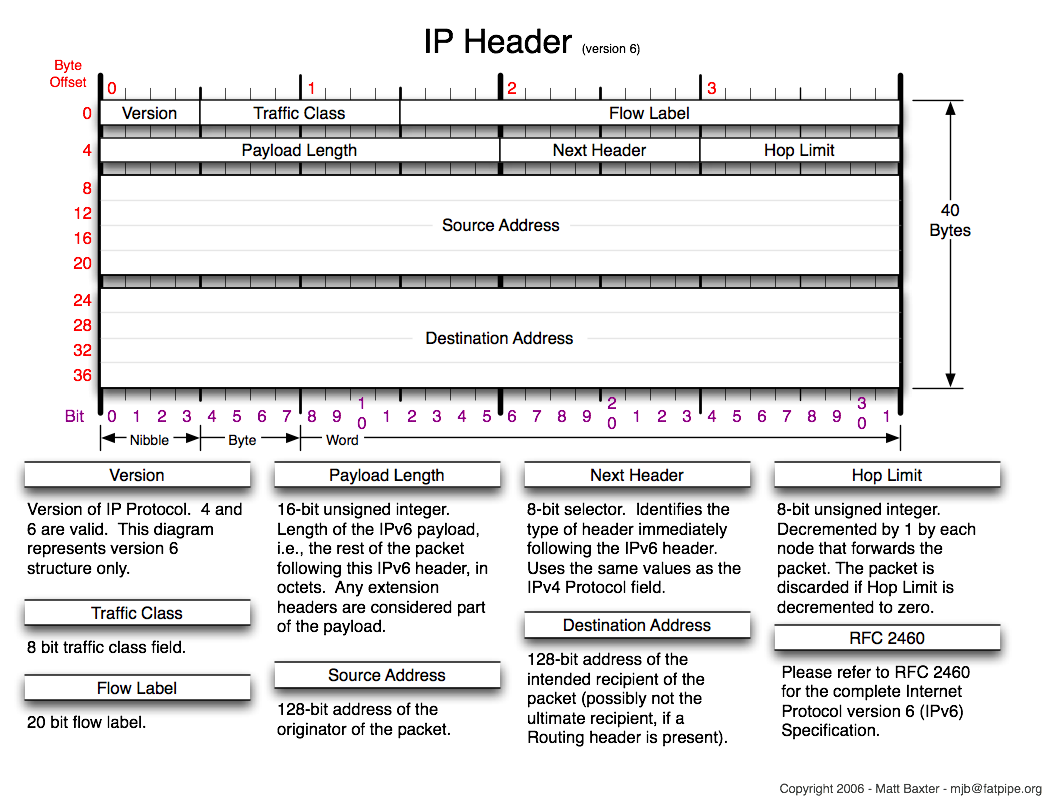
\includegraphics[scale=0.45]{images/IPv6-Header.png}\\[1cm]}


\newpage


\section{Layer 2: Bridging and Switching}

\subsection{Layers 1 and 2}

\begin{description}
	\item[Layer 1] Repeaters, hubs. Same collision domain. Same link segment.
	\item[Layer 2] Bridges, switches. Same collision domain. Same link segment.
\end{description}
	
	
\subsection{Layer 2: MAC and LLC}

\begin{description}
	\item[MAC] Media Access Control. Work from IEEE 802.3\footnote{\url{http://en.wikipedia.org/wiki/IEEE_802.3}}.
	\item[CSMA/CD] Carrier Sense Multiple Access With Collision Detection. Ethernet is the most common.
	\begin{enumerate}
    	\item Is my frame ready for transmission? If yes, move to 2.
    	\item Is medium idle? If not, wait until it becomes ready.
    	\item Start transmitting.
    	\item Did a collision occur? If so, go to collision detected procedure.
    	\item Reset retransmission counters and end frame transmission.
	\end{enumerate}
	\item[LLC] Logical Link Control. Multiplexing mechanisms, flow control and error management. Interface between MAC and Network Layer.
\end{description}
	
\subsection{Frame Formats}

\centerline{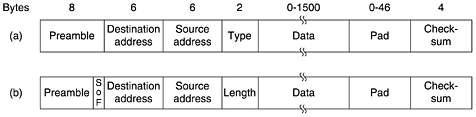
\includegraphics[scale=0.7]{images/Ethernet.png}\\[1cm]}

\begin{description}
	\item[DIX Ethernet] DEC-Intel-Xerox initial frame structure\footnote{\url{http://www.epubbud.com/read.php?g=5HEKFDZU&two=1&tocp=38}}.
	\begin{description}
    	\item[8bytes Preamble] Each one containing $10101010$. Used for synchronization.
    	\item[6bytes Destination Address]
    	\item[6bytes Source Address]
    	\item[2bytes Type] Indicator of the used transport protocol.
    	\item[0-1500bytes Payload]
    	\item[0-46bytes Pad] Valid Ethernet frames have, at least, 64 bytes (not counting Preamble!). If a frame is less than that (Payload < 46bytes), a pad is added to it. This is done to ease collision detection.
    	\item[4bytes Checksum] CRC of all the frame fields.
	\end{description}
	\item[802.3 Ethernet] Changes from DIX:
	\begin{description}
    	\item[7bytes Preamble + 1byte Start of Frame] Same as before but changing last byte to have compatibility with 802.4 and 802.5 (Token Bus and Token Ring).
    	\item[2bytes type -> 2bytes length] IEEE tried to change the purpose of the field (and move "type" information to *inside* the Payload), but some people did not change. Rule of thumb: if its value is over 1500, it is a Length field, otherwise it is a Type field.
    	\item[Changes on the Payload] There are 8 additional bytes of 'metadata' on the payload that are used mostly for nothing, effectively reducing the MTU from 1500 to 1492.
	\end{description}
	
\end{description}


\subsection{MAC Addresses}

\begin{description}
	\item[MAC48] Physical, obsolete.
	\item[EUI48] Virtual, including physical.
	\item[EUI64] Extended.
	\item[OUI] First 24bits of the MAC address. Identify who issued the device.
\end{description}


\subsection{EUI48 to EUI64}

[0:23bits]:FF:FE:[24:--bits]. When used to generate IPv6 address, the 7th most significative bit is swapped.

\subsection{Ethernet Types}

\begin{description}
	\item[0x0800] IP
	\item[0x0806] ARP
	\item[0x86DD] IPv6
\end{description}

\subsection{Bridges and Switches}

\begin{description}
	\item[Transparent Bridges] Use Store-and-Forward. Copy data from one port to another (or multiple ports). They can learn (and remember) where other devices are when they receive messages.
	\item[Switches are synonyms of Bridges] Usually refer to bridges with multiple interfaces.
\end{description}

\subsection{VLANs (802.1Q-2011)}

\centerline{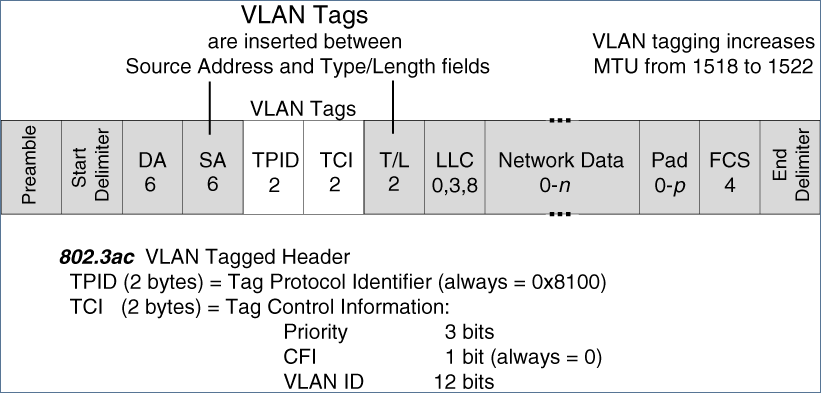
\includegraphics[scale=0.5]{images/VLAN.png}\\[1cm]}


\subsection{Layered Extensions}

TO-DO

\subsection{PBB-TE, TRILL, SPB}

TO-DO


\newpage









\section{STP Protocol}

\subsection{Goals and properties}

\begin{enumerate}
    \item Eliminate edges (connections) until there are no possible loops.
    \item After performing the algorithm, graph turns into a tree.
    \item Topology changes cause changes on the tree.
    \item Protocol works by electing a Root Node.
\end{enumerate}



\subsection{Configuration Messages}

\begin{description}
    \item[ID] based on a variable priority and its MAC address.
    \item[Root Node] Elected as the node with the lowest ID on the system.
    \item[Root ports on each Node] Chosen by\footnote{\url{https://www.youtube.com/watch?v=iB7BxtZVy3c}}:
    \begin{enumerate}
   		\item Lower advertised Root ID.
   		\item Lower advertised cost to Root.
   		\item Lower transmitting bridge ID.
   		\item Lower  port ID.
	\end{enumerate}
\end{description}

\centerline{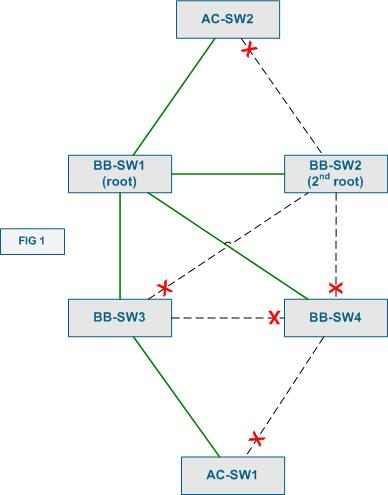
\includegraphics[scale=0.5]{images/STP-convergence.png}\\[1cm]}



\subsection{Timing Parameters}

\begin{description}
    \item[Hello Time] Time between two configuration messages.
    \item[Max Age] Parameter to discard messages that are too old.
    \item[Forward Delay] Half of the delay before transitioning from blocking to forwarding.
    \begin{enumerate}
   		\item Can be understood as two different waiting times. During that waiting, it does not forward packets.
   		\item First waiting: Listen for neighbours (other bridges).
   		\item Second waiting: Learn the location of MAC addresses.
	\end{enumerate}
\end{description}

\subsection{Topology Change Mechanism}


\begin{description}
   	\item[Memory] Bridges remember where other bridges are located.
   	\item[Stable Topology] When the topology is stable, bridges have a long caching time.
   	\item[Topology Changes] When a topology change is detected, the bridge detecting the change (and subsequent ones) sends a Topology Change Notification on his Root Port. When the message reaches the Root Bridge, it sets up its Topology Change flag. This causes other bridges to switch to the short caching delay.
\end{description}



\subsection{Bridge Protocol Data Unit (BPDU)}

\centerline{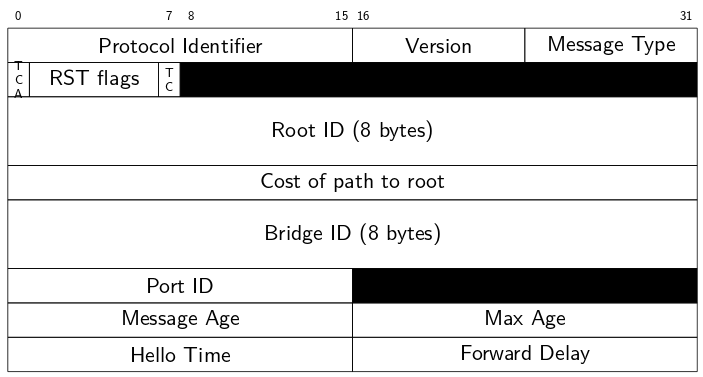
\includegraphics[scale=0.5]{images/BPDU.png}\\[1cm]}

\begin{description}
   	\item[Protocol Identifier] All zeroes.
   	\item[Version] 0 for STP, 2 for RST
   	\item[Message Type] 0 for Hello, 2 for RST, 128 for TCN
   	\item[Flags] TCA (Topology Change Ack), [Proposal, Agreement, ...], TC (Topology Change)
   	\item[Root ID]  Root Bridge.
   	\item[Cost to Root] Cost to the Root Bridge.
   	\item[Bridge ID] Bridge transmitting.
   	\item[Port ID] Port used on the transmitting bridge.
   	\item[Message Age] Age of the BPDU information.
   	\item[Max Age] Tipically 20 seconds (min 6).
   	\item[Hello Time] Tipically 2 seconds.
   	\item[Forward Delay] Tipically 15 seconds (min 4).
\end{description}

\subsection{STP Enhancements}

\begin{description}
   	\item[RST] 
   	\item[STP on VLANs]
   	\item[MSTP]
\end{description}




\newpage








\printbibliography

\end{document}
